% Options for packages loaded elsewhere
\PassOptionsToPackage{unicode}{hyperref}
\PassOptionsToPackage{hyphens}{url}
\PassOptionsToPackage{dvipsnames,svgnames,x11names}{xcolor}
%
\documentclass[
  letterpaper,
  DIV=11,
  numbers=noendperiod]{scrartcl}

\usepackage{amsmath,amssymb}
\usepackage{iftex}
\ifPDFTeX
  \usepackage[T1]{fontenc}
  \usepackage[utf8]{inputenc}
  \usepackage{textcomp} % provide euro and other symbols
\else % if luatex or xetex
  \usepackage{unicode-math}
  \defaultfontfeatures{Scale=MatchLowercase}
  \defaultfontfeatures[\rmfamily]{Ligatures=TeX,Scale=1}
\fi
\usepackage{lmodern}
\ifPDFTeX\else  
    % xetex/luatex font selection
\fi
% Use upquote if available, for straight quotes in verbatim environments
\IfFileExists{upquote.sty}{\usepackage{upquote}}{}
\IfFileExists{microtype.sty}{% use microtype if available
  \usepackage[]{microtype}
  \UseMicrotypeSet[protrusion]{basicmath} % disable protrusion for tt fonts
}{}
\makeatletter
\@ifundefined{KOMAClassName}{% if non-KOMA class
  \IfFileExists{parskip.sty}{%
    \usepackage{parskip}
  }{% else
    \setlength{\parindent}{0pt}
    \setlength{\parskip}{6pt plus 2pt minus 1pt}}
}{% if KOMA class
  \KOMAoptions{parskip=half}}
\makeatother
\usepackage{xcolor}
\setlength{\emergencystretch}{3em} % prevent overfull lines
\setcounter{secnumdepth}{5}
% Make \paragraph and \subparagraph free-standing
\ifx\paragraph\undefined\else
  \let\oldparagraph\paragraph
  \renewcommand{\paragraph}[1]{\oldparagraph{#1}\mbox{}}
\fi
\ifx\subparagraph\undefined\else
  \let\oldsubparagraph\subparagraph
  \renewcommand{\subparagraph}[1]{\oldsubparagraph{#1}\mbox{}}
\fi

\usepackage{color}
\usepackage{fancyvrb}
\newcommand{\VerbBar}{|}
\newcommand{\VERB}{\Verb[commandchars=\\\{\}]}
\DefineVerbatimEnvironment{Highlighting}{Verbatim}{commandchars=\\\{\}}
% Add ',fontsize=\small' for more characters per line
\usepackage{framed}
\definecolor{shadecolor}{RGB}{241,243,245}
\newenvironment{Shaded}{\begin{snugshade}}{\end{snugshade}}
\newcommand{\AlertTok}[1]{\textcolor[rgb]{0.68,0.00,0.00}{#1}}
\newcommand{\AnnotationTok}[1]{\textcolor[rgb]{0.37,0.37,0.37}{#1}}
\newcommand{\AttributeTok}[1]{\textcolor[rgb]{0.40,0.45,0.13}{#1}}
\newcommand{\BaseNTok}[1]{\textcolor[rgb]{0.68,0.00,0.00}{#1}}
\newcommand{\BuiltInTok}[1]{\textcolor[rgb]{0.00,0.23,0.31}{#1}}
\newcommand{\CharTok}[1]{\textcolor[rgb]{0.13,0.47,0.30}{#1}}
\newcommand{\CommentTok}[1]{\textcolor[rgb]{0.37,0.37,0.37}{#1}}
\newcommand{\CommentVarTok}[1]{\textcolor[rgb]{0.37,0.37,0.37}{\textit{#1}}}
\newcommand{\ConstantTok}[1]{\textcolor[rgb]{0.56,0.35,0.01}{#1}}
\newcommand{\ControlFlowTok}[1]{\textcolor[rgb]{0.00,0.23,0.31}{#1}}
\newcommand{\DataTypeTok}[1]{\textcolor[rgb]{0.68,0.00,0.00}{#1}}
\newcommand{\DecValTok}[1]{\textcolor[rgb]{0.68,0.00,0.00}{#1}}
\newcommand{\DocumentationTok}[1]{\textcolor[rgb]{0.37,0.37,0.37}{\textit{#1}}}
\newcommand{\ErrorTok}[1]{\textcolor[rgb]{0.68,0.00,0.00}{#1}}
\newcommand{\ExtensionTok}[1]{\textcolor[rgb]{0.00,0.23,0.31}{#1}}
\newcommand{\FloatTok}[1]{\textcolor[rgb]{0.68,0.00,0.00}{#1}}
\newcommand{\FunctionTok}[1]{\textcolor[rgb]{0.28,0.35,0.67}{#1}}
\newcommand{\ImportTok}[1]{\textcolor[rgb]{0.00,0.46,0.62}{#1}}
\newcommand{\InformationTok}[1]{\textcolor[rgb]{0.37,0.37,0.37}{#1}}
\newcommand{\KeywordTok}[1]{\textcolor[rgb]{0.00,0.23,0.31}{#1}}
\newcommand{\NormalTok}[1]{\textcolor[rgb]{0.00,0.23,0.31}{#1}}
\newcommand{\OperatorTok}[1]{\textcolor[rgb]{0.37,0.37,0.37}{#1}}
\newcommand{\OtherTok}[1]{\textcolor[rgb]{0.00,0.23,0.31}{#1}}
\newcommand{\PreprocessorTok}[1]{\textcolor[rgb]{0.68,0.00,0.00}{#1}}
\newcommand{\RegionMarkerTok}[1]{\textcolor[rgb]{0.00,0.23,0.31}{#1}}
\newcommand{\SpecialCharTok}[1]{\textcolor[rgb]{0.37,0.37,0.37}{#1}}
\newcommand{\SpecialStringTok}[1]{\textcolor[rgb]{0.13,0.47,0.30}{#1}}
\newcommand{\StringTok}[1]{\textcolor[rgb]{0.13,0.47,0.30}{#1}}
\newcommand{\VariableTok}[1]{\textcolor[rgb]{0.07,0.07,0.07}{#1}}
\newcommand{\VerbatimStringTok}[1]{\textcolor[rgb]{0.13,0.47,0.30}{#1}}
\newcommand{\WarningTok}[1]{\textcolor[rgb]{0.37,0.37,0.37}{\textit{#1}}}

\providecommand{\tightlist}{%
  \setlength{\itemsep}{0pt}\setlength{\parskip}{0pt}}\usepackage{longtable,booktabs,array}
\usepackage{calc} % for calculating minipage widths
% Correct order of tables after \paragraph or \subparagraph
\usepackage{etoolbox}
\makeatletter
\patchcmd\longtable{\par}{\if@noskipsec\mbox{}\fi\par}{}{}
\makeatother
% Allow footnotes in longtable head/foot
\IfFileExists{footnotehyper.sty}{\usepackage{footnotehyper}}{\usepackage{footnote}}
\makesavenoteenv{longtable}
\usepackage{graphicx}
\makeatletter
\def\maxwidth{\ifdim\Gin@nat@width>\linewidth\linewidth\else\Gin@nat@width\fi}
\def\maxheight{\ifdim\Gin@nat@height>\textheight\textheight\else\Gin@nat@height\fi}
\makeatother
% Scale images if necessary, so that they will not overflow the page
% margins by default, and it is still possible to overwrite the defaults
% using explicit options in \includegraphics[width, height, ...]{}
\setkeys{Gin}{width=\maxwidth,height=\maxheight,keepaspectratio}
% Set default figure placement to htbp
\makeatletter
\def\fps@figure{htbp}
\makeatother
\newlength{\cslhangindent}
\setlength{\cslhangindent}{1.5em}
\newlength{\csllabelwidth}
\setlength{\csllabelwidth}{3em}
\newlength{\cslentryspacingunit} % times entry-spacing
\setlength{\cslentryspacingunit}{\parskip}
\newenvironment{CSLReferences}[2] % #1 hanging-ident, #2 entry spacing
 {% don't indent paragraphs
  \setlength{\parindent}{0pt}
  % turn on hanging indent if param 1 is 1
  \ifodd #1
  \let\oldpar\par
  \def\par{\hangindent=\cslhangindent\oldpar}
  \fi
  % set entry spacing
  \setlength{\parskip}{#2\cslentryspacingunit}
 }%
 {}
\usepackage{calc}
\newcommand{\CSLBlock}[1]{#1\hfill\break}
\newcommand{\CSLLeftMargin}[1]{\parbox[t]{\csllabelwidth}{#1}}
\newcommand{\CSLRightInline}[1]{\parbox[t]{\linewidth - \csllabelwidth}{#1}\break}
\newcommand{\CSLIndent}[1]{\hspace{\cslhangindent}#1}

\KOMAoption{captions}{tableheading}
\makeatletter
\@ifpackageloaded{tcolorbox}{}{\usepackage[skins,breakable]{tcolorbox}}
\@ifpackageloaded{fontawesome5}{}{\usepackage{fontawesome5}}
\definecolor{quarto-callout-color}{HTML}{909090}
\definecolor{quarto-callout-note-color}{HTML}{0758E5}
\definecolor{quarto-callout-important-color}{HTML}{CC1914}
\definecolor{quarto-callout-warning-color}{HTML}{EB9113}
\definecolor{quarto-callout-tip-color}{HTML}{00A047}
\definecolor{quarto-callout-caution-color}{HTML}{FC5300}
\definecolor{quarto-callout-color-frame}{HTML}{acacac}
\definecolor{quarto-callout-note-color-frame}{HTML}{4582ec}
\definecolor{quarto-callout-important-color-frame}{HTML}{d9534f}
\definecolor{quarto-callout-warning-color-frame}{HTML}{f0ad4e}
\definecolor{quarto-callout-tip-color-frame}{HTML}{02b875}
\definecolor{quarto-callout-caution-color-frame}{HTML}{fd7e14}
\makeatother
\makeatletter
\makeatother
\makeatletter
\makeatother
\makeatletter
\@ifpackageloaded{caption}{}{\usepackage{caption}}
\AtBeginDocument{%
\ifdefined\contentsname
  \renewcommand*\contentsname{Table of contents}
\else
  \newcommand\contentsname{Table of contents}
\fi
\ifdefined\listfigurename
  \renewcommand*\listfigurename{List of Figures}
\else
  \newcommand\listfigurename{List of Figures}
\fi
\ifdefined\listtablename
  \renewcommand*\listtablename{List of Tables}
\else
  \newcommand\listtablename{List of Tables}
\fi
\ifdefined\figurename
  \renewcommand*\figurename{Figure}
\else
  \newcommand\figurename{Figure}
\fi
\ifdefined\tablename
  \renewcommand*\tablename{Table}
\else
  \newcommand\tablename{Table}
\fi
}
\@ifpackageloaded{float}{}{\usepackage{float}}
\floatstyle{ruled}
\@ifundefined{c@chapter}{\newfloat{codelisting}{h}{lop}}{\newfloat{codelisting}{h}{lop}[chapter]}
\floatname{codelisting}{Listing}
\newcommand*\listoflistings{\listof{codelisting}{List of Listings}}
\makeatother
\makeatletter
\@ifpackageloaded{caption}{}{\usepackage{caption}}
\@ifpackageloaded{subcaption}{}{\usepackage{subcaption}}
\makeatother
\makeatletter
\@ifpackageloaded{tcolorbox}{}{\usepackage[skins,breakable]{tcolorbox}}
\makeatother
\makeatletter
\@ifundefined{shadecolor}{\definecolor{shadecolor}{rgb}{.97, .97, .97}}
\makeatother
\makeatletter
\makeatother
\makeatletter
\makeatother
\ifLuaTeX
  \usepackage{selnolig}  % disable illegal ligatures
\fi
\IfFileExists{bookmark.sty}{\usepackage{bookmark}}{\usepackage{hyperref}}
\IfFileExists{xurl.sty}{\usepackage{xurl}}{} % add URL line breaks if available
\urlstyle{same} % disable monospaced font for URLs
\hypersetup{
  pdftitle={How I use ggplot2},
  colorlinks=true,
  linkcolor={blue},
  filecolor={Maroon},
  citecolor={Blue},
  urlcolor={Blue},
  pdfcreator={LaTeX via pandoc}}

\title{How I use ggplot2}
\author{Paul Schmidt}
\date{2023-07-24}

\begin{document}
\maketitle
\begin{abstract}
A brief introduction to ggplot2. Be warned: This chapter provides
detailed insight into certain aspects, while other components are not
discussed at all.
\end{abstract}
\ifdefined\Shaded\renewenvironment{Shaded}{\begin{tcolorbox}[sharp corners, breakable, frame hidden, enhanced, borderline west={3pt}{0pt}{shadecolor}, interior hidden, boxrule=0pt]}{\end{tcolorbox}}\fi

\renewcommand*\contentsname{Table of contents}
{
\hypersetup{linkcolor=}
\setcounter{tocdepth}{3}
\tableofcontents
}
\hypertarget{before-we-start}{%
\section{Before we start}\label{before-we-start}}

\hypertarget{who-this-is-for}{%
\subsection{Who this is for}\label{who-this-is-for}}

This tutorial serves as an introductory guide to ggplot2, tailored
specifically for beginners with no prior exposure to ggplot2. However,
it's worth mentioning that as we delve deeper into the subject, we'll
employ both BaseR and tidyverse code for some data preparations.

In addition, this ggplot2 guide reflects my personal approach and
application of visualization techniques, focusing on the disciplines
that align with the theme of this website - from agricultural sciences
to experimental data from biology or life sciences at large. This
tutorial, therefore, may not encompass all facets of ggplot2, but rather
those elements that I frequently utilize in these specific domains.

\hypertarget{other-resources}{%
\subsection{Other resources}\label{other-resources}}

Here are some other ggplot2 tutorials and resources that I like:

\begin{itemize}
\tightlist
\item
  \href{https://r4ds.had.co.nz/data-visualisation.html}{Chapter 3: Data
  Visualisation} in (Wickham and Grolemund 2017)
\item
  Cédric Scherer's (2022a)
  \href{https://www.cedricscherer.com/2019/08/05/a-ggplot2-tutorial-for-beautiful-plotting-in-r/}{A
  ggplot2 tutorial for beautiful plotting in R}
\item
  Cédric Scherer's (2022b)
  \href{https://rstudio-conf-2022.github.io/ggplot2-graphic-design/}{Graphic
  Design with ggplot2}
\item
  Andrew Heiss' (2023)
  \href{https://datavizs23.classes.andrewheiss.com/content/01-content.html}{Data
  visualization with R}
\item
  Claus Wilke's (2019)
  \href{https://clauswilke.com/dataviz/}{Fundamentals of Data
  Visualization}
\end{itemize}

\hypertarget{packages-to-install-load}{%
\subsection{Packages to install \&
load}\label{packages-to-install-load}}

We are using \href{../misc/usefulthings.html\#pacman}{the
\texttt{p\_load()} function of the \{pacman\} package} to install and
load all necessary packages for this tutorial.

\begin{Shaded}
\begin{Highlighting}[]
\NormalTok{pacman}\SpecialCharTok{::}\FunctionTok{p\_load}\NormalTok{(}
\NormalTok{  ggplot2,}
\NormalTok{  ggrepel,}
\NormalTok{  ggtext}
\NormalTok{  )}
\end{Highlighting}
\end{Shaded}

\hypertarget{showcase}{%
\subsection{Showcase}\label{showcase}}

Here are some beautiful ggplots

\hypertarget{lets-start}{%
\section{Let's start}\label{lets-start}}

Let us start by creating a plot that requires a minimum amount of code,
but is still informative. We make use the \texttt{PlantGrowth} data,
which is directly accessible in R.

\begin{Shaded}
\begin{Highlighting}[]
\FunctionTok{ggplot}\NormalTok{(}\AttributeTok{data =}\NormalTok{ PlantGrowth, }
       \AttributeTok{mapping =} \FunctionTok{aes}\NormalTok{(}\AttributeTok{y =}\NormalTok{ weight, }\AttributeTok{x =}\NormalTok{ group)) }\SpecialCharTok{+}
  \FunctionTok{geom\_point}\NormalTok{()}
\end{Highlighting}
\end{Shaded}

\begin{figure}[H]

{\centering 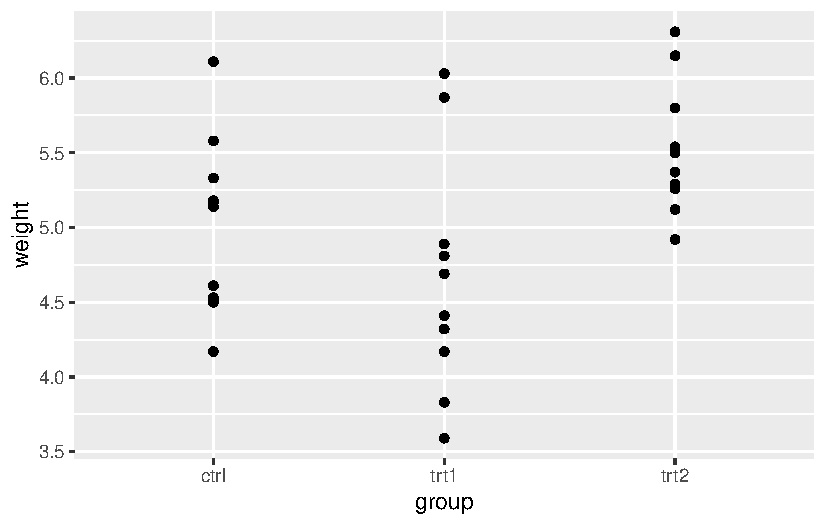
\includegraphics{ggplot2intro_files/figure-pdf/unnamed-chunk-3-1.pdf}

}

\end{figure}

\begin{Shaded}
\begin{Highlighting}[]
\FunctionTok{ggplot}\NormalTok{(}\AttributeTok{data =}\NormalTok{ PlantGrowth) }\SpecialCharTok{+}
  \FunctionTok{aes}\NormalTok{(}\AttributeTok{y =}\NormalTok{ weight, }\AttributeTok{x =}\NormalTok{ group) }\SpecialCharTok{+}
  \FunctionTok{geom\_point}\NormalTok{()}
\end{Highlighting}
\end{Shaded}

\begin{figure}[H]

{\centering 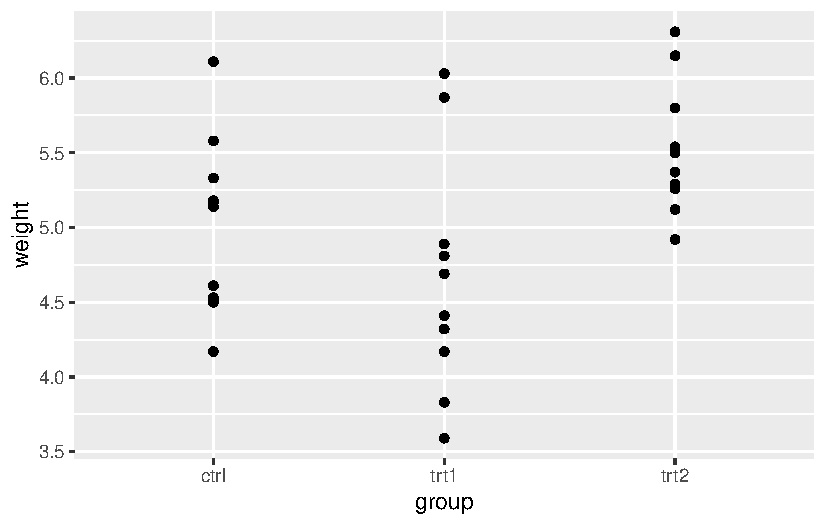
\includegraphics{ggplot2intro_files/figure-pdf/unnamed-chunk-4-1.pdf}

}

\end{figure}

Actually, you can see we created the same plot twice using slightly
different code. Apologies for immediately confusing you with this, but
it would be even more confusing if we postpone this topic.

Let's try to understand the general approach by looking at the first
version of the code. The code for any ggplot always starts with the
\texttt{ggplot()} function and then \textbf{layers} are added to it via
the \texttt{+} operator.

The \texttt{data\ =} argument in \texttt{ggplot()} is where you specify
the dataset you want to visualize. Think of it as telling ggplot ``Here
is the data I want you to work with.''

The \texttt{mapping\ =\ aes()} argument is where you define the
aesthetic mappings, like which columns of the data should be represented
on the x and y axes. It's like giving ggplot specific instructions on
``How should you represent this data?'' For instance,
\texttt{mapping\ =\ aes(x\ =\ column1,\ y\ =\ column2)} would tell
ggplot to use \texttt{column1} for the x-axis and \texttt{column2} for
the y-axis.

So, together, these two arguments form the fundamental instructions for
any ggplot: ``Here is my data, and this is how I want you to represent
it.''

Looking at our two versions of code that result in the same plot, you
can see that they only differ in how the \texttt{aes()} is included. The
far more common approach is to include it inside the \texttt{ggplot()}
function as in the first version. However, I am
\href{https://twitter.com/sharoz/status/1559925104645136386}{not the
only one} who argues that the second version is simply easier to read,
which is why I am using it. Other than that, there is no difference
between the two versions.

Finally, there is \texttt{geom\_point()}. This function, known as a
geometric object or ``geom'', represents the type of plot you want to
create. In ggplot2, every type of plot is associated with a specific
geom function. For our example,\texttt{geom\_point()} is used to create
a scatter plot, draws a point for each observation. The
\texttt{geom\_point()} function is added to the base \texttt{ggplot()}
call using the \texttt{+} operator, just like the other layers. In this
way, it's as if we're telling ggplot: ``And here is the type of plot I
want you to create.''. Again - it already knows \emph{where} to draw the
points because we told it about the data and aesthetic mapping.

Other geoms you might use include \texttt{geom\_boxplot()} for boxplots,
\texttt{geom\_line()} for line graphs, and
\href{https://ggplot2.tidyverse.org/reference/\#geoms}{many more}. Each
geom function has its own set of aesthetics and other arguments that you
can specify to customize your plot. By using these different geoms, you
can create a wide variety of plots to meet your specific data
visualization needs.

Now you understand the absolute minimum of how to create a ggplot.

\begin{tcolorbox}[enhanced jigsaw, left=2mm, title=\textcolor{quarto-callout-tip-color}{\faLightbulb}\hspace{0.5em}{Additional Resources}, toprule=.15mm, colback=white, coltitle=black, opacityback=0, breakable, titlerule=0mm, bottomtitle=1mm, toptitle=1mm, colbacktitle=quarto-callout-tip-color!10!white, arc=.35mm, rightrule=.15mm, bottomrule=.15mm, leftrule=.75mm, colframe=quarto-callout-tip-color-frame, opacitybacktitle=0.6]

\begin{itemize}
\tightlist
\item
  \href{https://ggplot2.tidyverse.org/reference/\#geoms}{List of all
  \texttt{geom\_*()} functons}
\end{itemize}

\end{tcolorbox}

\hypertarget{saving-and-reusing-plots}{%
\section{Saving and reusing plots}\label{saving-and-reusing-plots}}

In ggplot2, you can save your plots into an object. This allows you to
reuse and modify your plots without having to rewrite all the code. This
is particularly useful when you are building complex plots layer by
layer.

Let's take the plot we have created so far. Instead of writing the code
for all the layers every time, we can save the plot into an object and
then add new layers to this object. This way, we can focus on the new
layers we are adding, making our code more readable and manageable.

Here's how we can do this:

\begin{Shaded}
\begin{Highlighting}[]
\NormalTok{myplot }\OtherTok{\textless{}{-}} \FunctionTok{ggplot}\NormalTok{(}\AttributeTok{data =}\NormalTok{ PlantGrowth) }\SpecialCharTok{+}
  \FunctionTok{aes}\NormalTok{(}\AttributeTok{y =}\NormalTok{ weight, }\AttributeTok{x =}\NormalTok{ group) }\SpecialCharTok{+}
  \FunctionTok{geom\_point}\NormalTok{()}
\end{Highlighting}
\end{Shaded}

Be aware that when running this code, you will not get to see the plot
you just saved. Instead, you would need to run the \texttt{myplot}
object to see the plot:

\begin{Shaded}
\begin{Highlighting}[]
\NormalTok{myplot}
\end{Highlighting}
\end{Shaded}

\begin{figure}[H]

{\centering 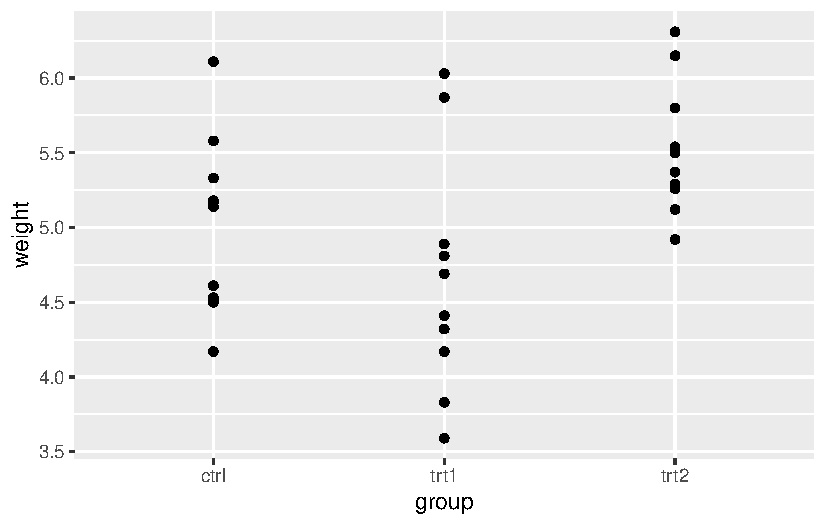
\includegraphics{ggplot2intro_files/figure-pdf/unnamed-chunk-6-1.pdf}

}

\end{figure}

This approach of saving and reusing plots not only makes our code more
readable and manageable, but also allows us to experiment with different
layers and modifications without affecting our original plot.

From now on, we will use this approach in our tutorial. At the end of
each main section, we will update \texttt{myplot} with the new layers we
have discussed in that section. This will allow us to build our plot
step by step, focusing on one aspect at a time.

\hypertarget{axes}{%
\section{Axes}\label{axes}}

In ggplot2, the \texttt{scale\_x\_*} and \texttt{scale\_y\_*} functions
are used to control the appearance of the x and y axes, respectively.
These functions allow you to set the scale type (continuous, discrete,
etc.), the axis labels, the tick mark labels, and the range of values
displayed on the axis.

Regarding the scale type, we need to use \texttt{scale\_y\_continuous()}
(since \texttt{weight} is a continous, metric variable) and
\texttt{scale\_x\_discrete()} (since \texttt{group} is a discrete,
categorical variable) for our scatter plot.

\hypertarget{name}{%
\subsection{Name}\label{name}}

The \texttt{name\ =} allows you to change the axis titles.

\begin{Shaded}
\begin{Highlighting}[]
\NormalTok{myplot }\SpecialCharTok{+}
  \FunctionTok{scale\_y\_continuous}\NormalTok{(}\AttributeTok{name =} \StringTok{"Weight (g)"}\NormalTok{) }\SpecialCharTok{+}
  \FunctionTok{scale\_x\_discrete}\NormalTok{(}\AttributeTok{name =} \StringTok{"Treatment Group"}\NormalTok{)}
\end{Highlighting}
\end{Shaded}

\begin{figure}[H]

{\centering 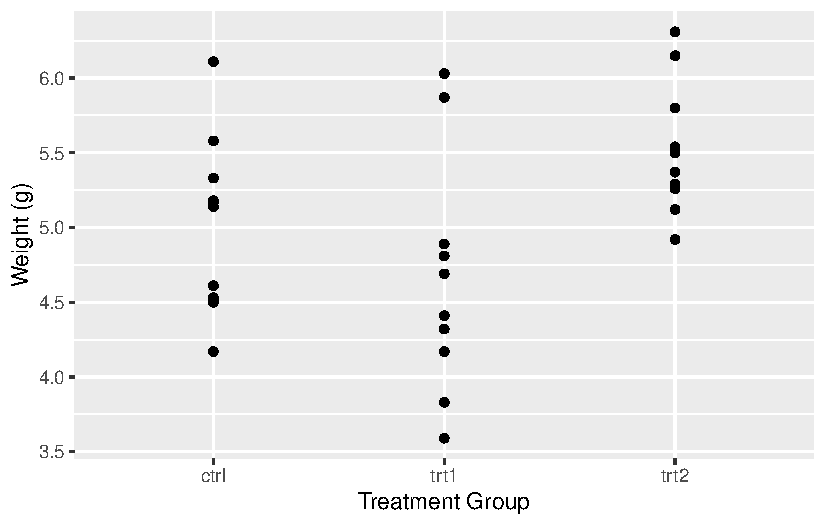
\includegraphics{ggplot2intro_files/figure-pdf/unnamed-chunk-7-1.pdf}

}

\end{figure}

\hypertarget{limits}{%
\subsection{Limits}\label{limits}}

The \texttt{limits\ =} argument in the scale\_*\_* functions allows you
to specify the range of values displayed on the axis. This can be
particularly useful when you want to focus on a specific part of your
data. Let's see how this works in practice with our scatter plot
example.

\begin{Shaded}
\begin{Highlighting}[]
\NormalTok{myplot }\SpecialCharTok{+}
  \FunctionTok{scale\_y\_continuous}\NormalTok{(}
    \AttributeTok{name =} \StringTok{"Weight (g)"}\NormalTok{,}
    \AttributeTok{limits =} \FunctionTok{c}\NormalTok{(}\DecValTok{0}\NormalTok{, }\DecValTok{7}\NormalTok{)}
\NormalTok{  ) }\SpecialCharTok{+}
  \FunctionTok{scale\_x\_discrete}\NormalTok{(}
    \AttributeTok{name =} \StringTok{"Treatment Group"}\NormalTok{,}
    \AttributeTok{limits =} \FunctionTok{c}\NormalTok{(}\StringTok{"ctrl"}\NormalTok{, }\StringTok{"trt2"}\NormalTok{)}
\NormalTok{  )}
\end{Highlighting}
\end{Shaded}

\begin{figure}[H]

{\centering 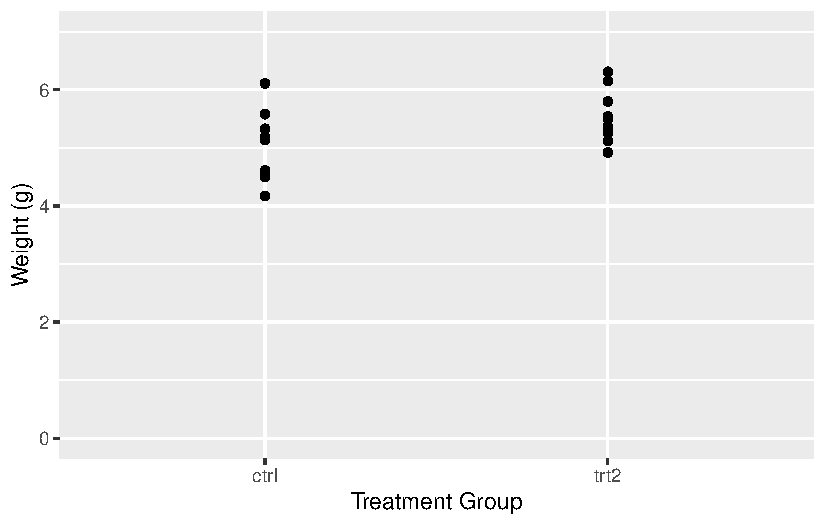
\includegraphics{ggplot2intro_files/figure-pdf/unnamed-chunk-8-1.pdf}

}

\end{figure}

\begin{Shaded}
\begin{Highlighting}[]
\NormalTok{myplot }\SpecialCharTok{+}
  \FunctionTok{scale\_y\_continuous}\NormalTok{(}
    \AttributeTok{name =} \StringTok{"Weight (g)"}\NormalTok{,}
    \AttributeTok{limits =} \FunctionTok{c}\NormalTok{(}\DecValTok{0}\NormalTok{, }\ConstantTok{NA}\NormalTok{)}
\NormalTok{  ) }\SpecialCharTok{+}
  \FunctionTok{scale\_x\_discrete}\NormalTok{(}
    \AttributeTok{name =} \StringTok{"Treatment Group"}\NormalTok{,}
    \AttributeTok{limits =} \FunctionTok{c}\NormalTok{(}\StringTok{"trt1"}\NormalTok{, }\StringTok{"ctrl"}\NormalTok{, }\StringTok{"trt2"}\NormalTok{)}
\NormalTok{  )}
\end{Highlighting}
\end{Shaded}

\begin{figure}[H]

{\centering 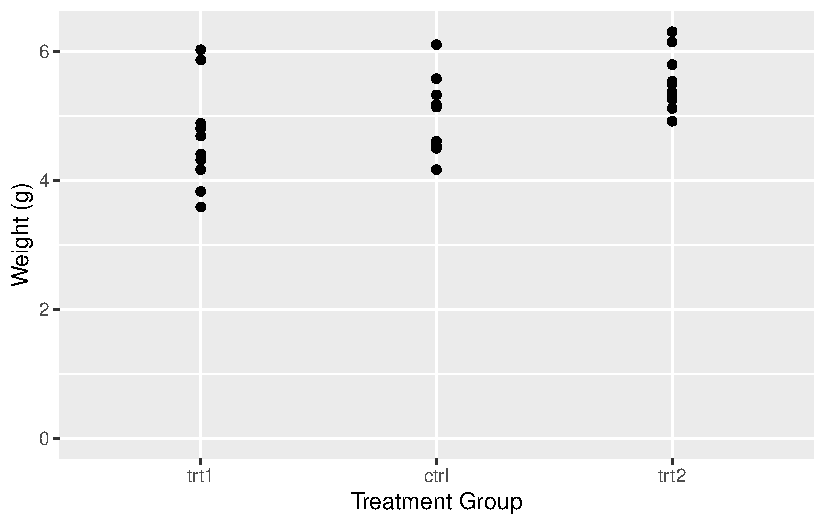
\includegraphics{ggplot2intro_files/figure-pdf/unnamed-chunk-9-1.pdf}

}

\end{figure}

In the left plot, we use the \texttt{limits\ =} argument in
\texttt{scale\_y\_continuous()} to set the y-axis to range from 0 to 7.
This works as expected, showing all weights from 0 to 7. However,
including only ``ctrl'' and ``trt2'' (i.e.~the first and last level) in
the \texttt{limits\ =} argument of in \texttt{scale\_x\_discrete()},
results in only these two groups being displayed on the x-axis. The key
point here is that for a discrete scale, the \texttt{limits\ =} argument
needs to include all the levels you want to display.

In the right plot, we again use the \texttt{limits\ =} argument in
\texttt{scale\_y\_continuous()}, but this time we only specify the lower
limit (0) and use \texttt{NA} for the upper limit. This tells ggplot2 to
start the y-axis at 0 and end it at the maximum value in the data, which
is the default behavior. For the x-axis, we provide all three levels
(``trt1'', ``ctrl'', ``trt2'') in the \texttt{limits\ =} argument of
\texttt{scale\_x\_discrete()}. This not only ensures that all groups are
displayed, but also allows us to control the order in which they appear.

This demonstrates how the \texttt{limits\ =} argument can be used
differently in \texttt{scale\_*\_continuous()} and
\texttt{scale\_*\_discrete()}. In a continuous scale, it defines the
range of values, while in a discrete scale, it specifies which levels to
include and their order.

In the end, it's important to note that setting the limits can exclude
data outside the specified range from the plot. This means that the
excluded data will not be considered when calculating statistics or
generating geoms. In other words, while setting limits can help focus
your plot on specific aspects of your data, it can also exclude
important information. Always consider the implications of setting
limits on your data visualization.

\begin{tcolorbox}[enhanced jigsaw, left=2mm, title=\textcolor{quarto-callout-tip-color}{\faLightbulb}\hspace{0.5em}{Additional Resources}, toprule=.15mm, colback=white, coltitle=black, opacityback=0, breakable, titlerule=0mm, bottomtitle=1mm, toptitle=1mm, colbacktitle=quarto-callout-tip-color!10!white, arc=.35mm, rightrule=.15mm, bottomrule=.15mm, leftrule=.75mm, colframe=quarto-callout-tip-color-frame, opacitybacktitle=0.6]

\begin{itemize}
\tightlist
\item
  If you are wondering why I wanted the y-axis to start at 0, read
  \href{https://academy.datawrapper.de/article/326-why-our-column-and-bar-charts-start-at-zero}{this},
  \href{https://digitalblog.ons.gov.uk/2016/06/27/does-the-axis-have-to-start-at-zero-part-1-line-charts/}{this}
  and
  \href{https://stats.stackexchange.com/questions/184525/how-to-determine-whether-or-not-the-y-axis-of-a-graph-should-start-at-zero}{this}
\item
  \href{https://ggplot2.tidyverse.org/reference/index.html\#scales}{List
  of all scales functions}
\end{itemize}

\end{tcolorbox}

\hypertarget{breaks}{%
\subsection{Breaks}\label{breaks}}

The breaks = argument in these functions allows you to specify the
locations of the tick marks on the axis.

\begin{Shaded}
\begin{Highlighting}[]
\NormalTok{myplot }\SpecialCharTok{+}
  \FunctionTok{scale\_y\_continuous}\NormalTok{(}
    \AttributeTok{name =} \StringTok{"Weight (g)"}\NormalTok{,}
    \AttributeTok{limits =} \FunctionTok{c}\NormalTok{(}\DecValTok{0}\NormalTok{, }\ConstantTok{NA}\NormalTok{),}
    \AttributeTok{breaks =} \FunctionTok{c}\NormalTok{(}\DecValTok{0}\NormalTok{, }\DecValTok{6}\NormalTok{)}
\NormalTok{  ) }\SpecialCharTok{+}
  \FunctionTok{scale\_x\_discrete}\NormalTok{(}
    \AttributeTok{name =} \StringTok{"Treatment Group"}
\NormalTok{  )}
\end{Highlighting}
\end{Shaded}

\begin{figure}[H]

{\centering 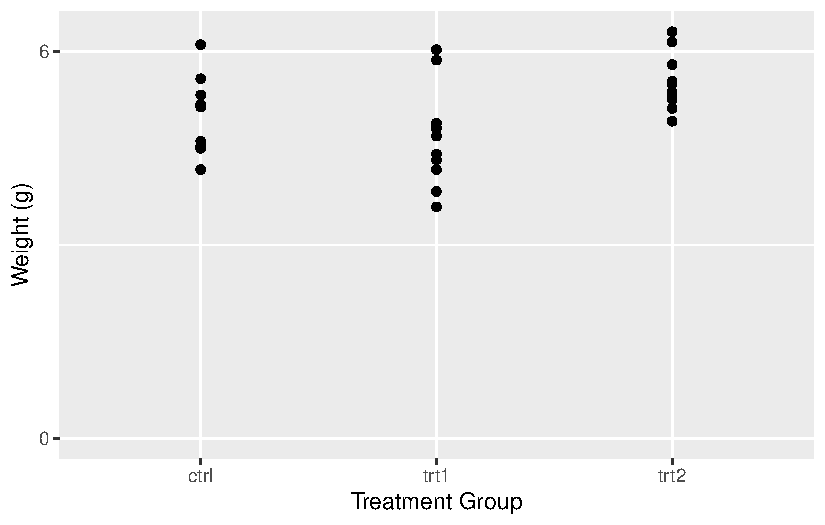
\includegraphics{ggplot2intro_files/figure-pdf/unnamed-chunk-10-1.pdf}

}

\end{figure}

\begin{Shaded}
\begin{Highlighting}[]
\NormalTok{myplot }\SpecialCharTok{+}
  \FunctionTok{scale\_y\_continuous}\NormalTok{(}
    \AttributeTok{name =} \StringTok{"Weight (g)"}\NormalTok{,}
    \AttributeTok{limits =} \FunctionTok{c}\NormalTok{(}\DecValTok{0}\NormalTok{, }\ConstantTok{NA}\NormalTok{),}
    \AttributeTok{breaks =} \FunctionTok{seq}\NormalTok{(}\DecValTok{0}\NormalTok{, }\DecValTok{6}\NormalTok{)}
\NormalTok{  ) }\SpecialCharTok{+}
  \FunctionTok{scale\_x\_discrete}\NormalTok{(}
    \AttributeTok{name =} \StringTok{"Treatment Group"}
\NormalTok{  )}
\end{Highlighting}
\end{Shaded}

\begin{figure}[H]

{\centering 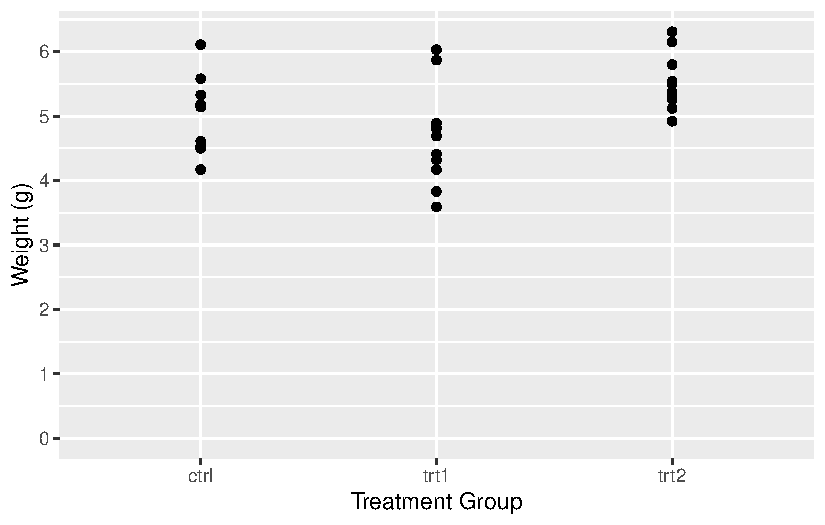
\includegraphics{ggplot2intro_files/figure-pdf/unnamed-chunk-11-1.pdf}

}

\end{figure}

In the left plot, we use the \texttt{breaks\ =} argument in
\texttt{scale\_y\_continuous()} to set the y-axis tick marks at 0 and 6.
This really results in only two tick marks being displayed on the
y-axis. While this is not typically useful for data representation, it
serves to illustrate that the \texttt{breaks\ =} argument can be used to
place tick marks at any specified values.

In the right plot, we use the \texttt{seq()} function in the
\texttt{breaks\ =} argument to set the y-axis tick marks at every
integer value from 0 to 6. This provides a more informative view of the
data, as it allows us to see the weight values at regular intervals.

\begin{tcolorbox}[enhanced jigsaw, left=2mm, title=\textcolor{quarto-callout-tip-color}{\faLightbulb}\hspace{0.5em}{Tip}, toprule=.15mm, colback=white, coltitle=black, opacityback=0, breakable, titlerule=0mm, bottomtitle=1mm, toptitle=1mm, colbacktitle=quarto-callout-tip-color!10!white, arc=.35mm, rightrule=.15mm, bottomrule=.15mm, leftrule=.75mm, colframe=quarto-callout-tip-color-frame, opacitybacktitle=0.6]

Instead of having to manually write ``6'' in
\texttt{breaks\ =\ seq(0,\ 6)} you can instead do this:

\begin{itemize}
\tightlist
\item
  \texttt{breaks\ =\ seq(0,\ max(PlantGrowth\$weight))} automatically
  finds the maximum value in the data
\item
  \texttt{breaks\ =\ scales::breaks\_width(1)} makes use of the
  \texttt{breaks\_width()} function in the
  \href{https://scales.r-lib.org/index.html}{\{scales\}} package to
  simply define the width of the breaks
\end{itemize}

\end{tcolorbox}

\hypertarget{labels}{%
\subsection{Labels}\label{labels}}

The \texttt{labels\ =} argument allows you to specify the text that is
displayed for each tick mark on the axis. This can be particularly
useful when the values in your data are not self-explanatory or when you
want to use more descriptive labels.

\begin{Shaded}
\begin{Highlighting}[]
\NormalTok{myplot }\SpecialCharTok{+}
  \FunctionTok{scale\_y\_continuous}\NormalTok{(}
    \AttributeTok{name =} \StringTok{"Weight (g)"}\NormalTok{,}
    \AttributeTok{limits =} \FunctionTok{c}\NormalTok{(}\DecValTok{0}\NormalTok{, }\ConstantTok{NA}\NormalTok{),}
    \AttributeTok{breaks =} \FunctionTok{seq}\NormalTok{(}\DecValTok{0}\NormalTok{, }\DecValTok{6}\NormalTok{)}
\NormalTok{  ) }\SpecialCharTok{+}
  \FunctionTok{scale\_x\_discrete}\NormalTok{(}
    \AttributeTok{name =} \StringTok{"Treatment Group"}\NormalTok{,}
    \AttributeTok{labels =} \FunctionTok{c}\NormalTok{(}\StringTok{"Control"}\NormalTok{, }\StringTok{"Treatment 1"}\NormalTok{, }\StringTok{"Treatment 2"}\NormalTok{)}
\NormalTok{  )}
\end{Highlighting}
\end{Shaded}

\begin{figure}[H]

{\centering 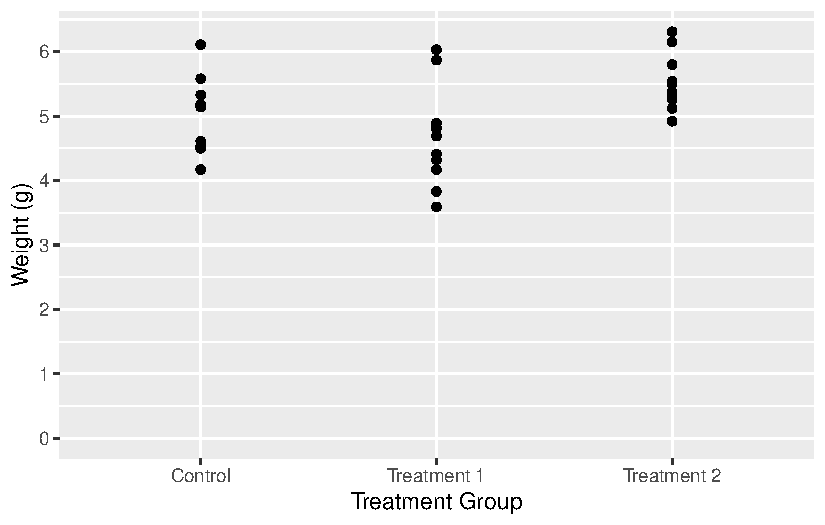
\includegraphics{ggplot2intro_files/figure-pdf/unnamed-chunk-12-1.pdf}

}

\end{figure}

\begin{Shaded}
\begin{Highlighting}[]
\NormalTok{myplot }\SpecialCharTok{+}
  \FunctionTok{scale\_y\_continuous}\NormalTok{(}
    \AttributeTok{name =} \StringTok{"Weight (g)"}\NormalTok{,}
    \AttributeTok{limits =} \FunctionTok{c}\NormalTok{(}\DecValTok{0}\NormalTok{, }\ConstantTok{NA}\NormalTok{),}
    \AttributeTok{breaks =} \FunctionTok{seq}\NormalTok{(}\DecValTok{0}\NormalTok{, }\DecValTok{6}\NormalTok{)}
\NormalTok{  ) }\SpecialCharTok{+}
  \FunctionTok{scale\_x\_discrete}\NormalTok{(}
    \AttributeTok{name =} \StringTok{"Treatment Group"}\NormalTok{,}
    \AttributeTok{labels =} \FunctionTok{c}\NormalTok{(}
      \AttributeTok{ctrl =} \StringTok{"Control"}\NormalTok{, }
      \AttributeTok{trt1 =} \StringTok{"Treatment 1"}\NormalTok{, }
      \AttributeTok{trt2 =} \StringTok{"Treatment 2"}
\NormalTok{    )}
\NormalTok{  )}
\end{Highlighting}
\end{Shaded}

\begin{figure}[H]

{\centering 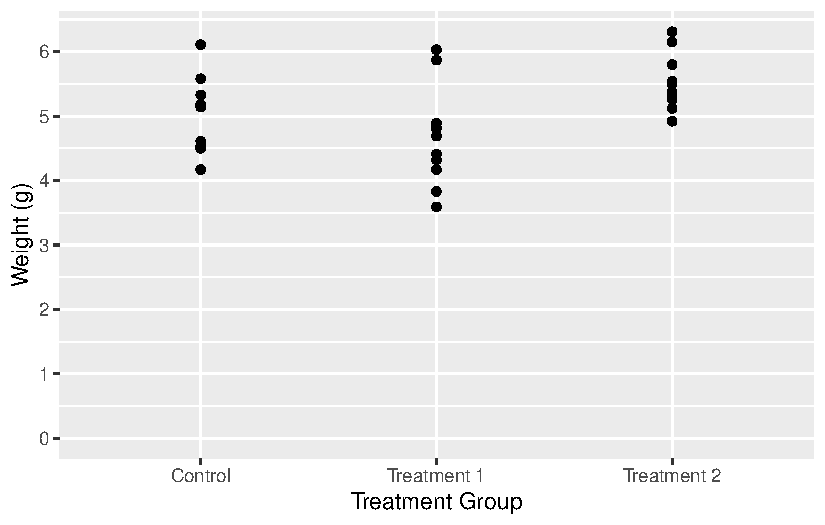
\includegraphics{ggplot2intro_files/figure-pdf/unnamed-chunk-13-1.pdf}

}

\end{figure}

In the first example, we simply provide a vector of labels. This works
fine as long as the levels on the x-axis are in the same order as the
labels in the vector. However, if the levels are not in the expected
order, the labels will be associated with the wrong levels.

In the second example, we provide a named vector of labels. This ensures
that the labels are correctly associated with their corresponding
levels, regardless of the order of the levels. This is why using a named
vector is often the safer option.

\begin{tcolorbox}[enhanced jigsaw, left=2mm, title=\textcolor{quarto-callout-tip-color}{\faLightbulb}\hspace{0.5em}{Tip}, toprule=.15mm, colback=white, coltitle=black, opacityback=0, breakable, titlerule=0mm, bottomtitle=1mm, toptitle=1mm, colbacktitle=quarto-callout-tip-color!10!white, arc=.35mm, rightrule=.15mm, bottomrule=.15mm, leftrule=.75mm, colframe=quarto-callout-tip-color-frame, opacitybacktitle=0.6]

You can also use \texttt{labels\ =} on continuous axes, if you make use
of the
\href{https://scales.r-lib.org/reference/index.html\#axis-labels}{\texttt{label\_*()}
functions} in the \href{https://scales.r-lib.org/index.html}{\{scales\}}
package. Here are some examples:

\begin{itemize}
\tightlist
\item
  \texttt{labels\ =\ label\_number()} displays numbers on your axis any
  way you want. E.g. \texttt{decimal.mark\ =\ "."} displays axis label
  3.14 as 3,14 etc.
\item
  \texttt{labels\ =\ label\_percent()} displays axis labels 0.05, 0.4 as
  5\%, 40\% etc.
\item
  \texttt{labels\ =\ label\_log()} displays axis labels 10, 100, 1000 as
  \(10^1\), \(10^2\), \(10^3\) etc.
\end{itemize}

\end{tcolorbox}

\hypertarget{expand}{%
\subsection{Expand}\label{expand}}

The \texttt{expand\ =} argument in the scale\_*\_* functions allows you
to control the expansion of the scale. This is particularly useful when
you want to adjust the space between the plotted data and the axes.

By default, ggplot2 adds a small amount of space around the data to
ensure that the data doesn't overlap with the axes. However, there might
be situations where you want to adjust this space. For instance, you
might want to remove the space below the 0 on the y-axis.

\begin{Shaded}
\begin{Highlighting}[]
\NormalTok{myplot }\SpecialCharTok{+}
  \FunctionTok{scale\_y\_continuous}\NormalTok{(}
    \AttributeTok{name =} \StringTok{"Weight (g)"}\NormalTok{,}
    \AttributeTok{limits =} \FunctionTok{c}\NormalTok{(}\DecValTok{0}\NormalTok{, }\ConstantTok{NA}\NormalTok{),}
    \AttributeTok{breaks =} \FunctionTok{seq}\NormalTok{(}\DecValTok{0}\NormalTok{, }\DecValTok{6}\NormalTok{),}
    \AttributeTok{expand =} \FunctionTok{c}\NormalTok{(}\DecValTok{0}\NormalTok{, }\DecValTok{0}\NormalTok{)}
\NormalTok{  ) }\SpecialCharTok{+}
  \FunctionTok{scale\_x\_discrete}\NormalTok{(}
    \AttributeTok{name =} \StringTok{"Treatment Group"}\NormalTok{,}
    \AttributeTok{labels =} \FunctionTok{c}\NormalTok{(}
      \AttributeTok{ctrl =} \StringTok{"Control"}\NormalTok{, }
      \AttributeTok{trt1 =} \StringTok{"Treatment 1"}\NormalTok{, }
      \AttributeTok{trt2 =} \StringTok{"Treatment 2"}
\NormalTok{    )}
\NormalTok{  )}
\end{Highlighting}
\end{Shaded}

\begin{figure}[H]

{\centering 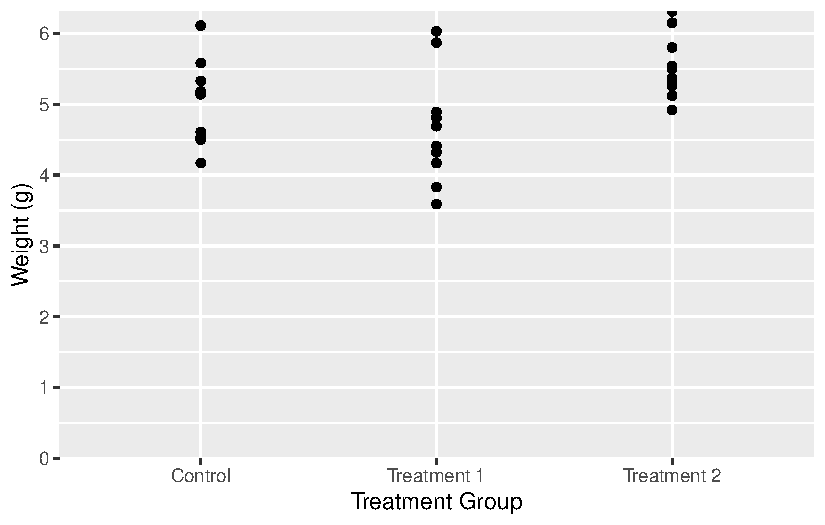
\includegraphics{ggplot2intro_files/figure-pdf/unnamed-chunk-14-1.pdf}

}

\end{figure}

\begin{Shaded}
\begin{Highlighting}[]
\NormalTok{myplot }\SpecialCharTok{+}
  \FunctionTok{scale\_y\_continuous}\NormalTok{(}
    \AttributeTok{name =} \StringTok{"Weight (g)"}\NormalTok{,}
    \AttributeTok{limits =} \FunctionTok{c}\NormalTok{(}\DecValTok{0}\NormalTok{, }\ConstantTok{NA}\NormalTok{),}
    \AttributeTok{breaks =} \FunctionTok{seq}\NormalTok{(}\DecValTok{0}\NormalTok{, }\DecValTok{6}\NormalTok{),}
    \AttributeTok{expand =} \FunctionTok{expansion}\NormalTok{(}\AttributeTok{mult =} \FunctionTok{c}\NormalTok{(}\DecValTok{0}\NormalTok{, }\FloatTok{0.05}\NormalTok{))}
\NormalTok{  ) }\SpecialCharTok{+}
  \FunctionTok{scale\_x\_discrete}\NormalTok{(}
    \AttributeTok{name =} \StringTok{"Treatment Group"}\NormalTok{,}
    \AttributeTok{labels =} \FunctionTok{c}\NormalTok{(}
      \AttributeTok{ctrl =} \StringTok{"Control"}\NormalTok{, }
      \AttributeTok{trt1 =} \StringTok{"Treatment 1"}\NormalTok{, }
      \AttributeTok{trt2 =} \StringTok{"Treatment 2"}
\NormalTok{    )}
\NormalTok{  )}
\end{Highlighting}
\end{Shaded}

\begin{figure}[H]

{\centering 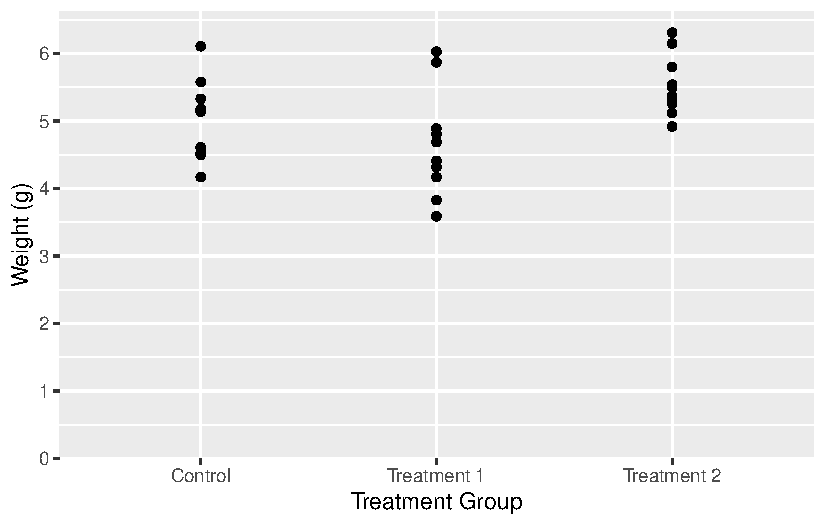
\includegraphics{ggplot2intro_files/figure-pdf/unnamed-chunk-15-1.pdf}

}

\end{figure}

In the left plot, we use the \texttt{expand\ =\ c(0,\ 0)} argument in
\texttt{scale\_y\_continuous()} to simply set the expansion to 0 on both
sides of the scale. This removes all extra space around the data.
However, this also results in the plot being cut off right at the
maximum observation, which might not be desirable.

In the right plot, we use the
\href{https://ggplot2.tidyverse.org/reference/expansion.html}{\texttt{expansion()}}
function in the \texttt{expand\ =} argument. This function allows us to
set different expansion multipliers for the lower and upper limits of
the scale. Here, we set the lower multiplier to 0 to remove the space
below 0, and the upper multiplier to 0.05 to add a small amount (= 5\%)
of space above the maximum observation.

\begin{tcolorbox}[enhanced jigsaw, left=2mm, title=\textcolor{quarto-callout-tip-color}{\faLightbulb}\hspace{0.5em}{Tip}, toprule=.15mm, colback=white, coltitle=black, opacityback=0, breakable, titlerule=0mm, bottomtitle=1mm, toptitle=1mm, colbacktitle=quarto-callout-tip-color!10!white, arc=.35mm, rightrule=.15mm, bottomrule=.15mm, leftrule=.75mm, colframe=quarto-callout-tip-color-frame, opacitybacktitle=0.6]

For a better understanding of how this expansion-thing works, I found
\href{https://twitter.com/ChBurkhart/status/1492087527511052290}{this
cheat sheet} to be insightful.

\end{tcolorbox}

We update our \texttt{myplot} according to what we just learned. To get
a better overview, we recreate it from scratch:

\begin{Shaded}
\begin{Highlighting}[]
\NormalTok{myplot }\OtherTok{\textless{}{-}} \FunctionTok{ggplot}\NormalTok{(}\AttributeTok{data =}\NormalTok{ PlantGrowth) }\SpecialCharTok{+}
  \FunctionTok{aes}\NormalTok{(}\AttributeTok{y =}\NormalTok{ weight, }\AttributeTok{x =}\NormalTok{ group) }\SpecialCharTok{+}
  \FunctionTok{geom\_point}\NormalTok{() }\SpecialCharTok{+}
  \FunctionTok{scale\_y\_continuous}\NormalTok{(}
    \AttributeTok{name =} \StringTok{"Weight (g)"}\NormalTok{,}
    \AttributeTok{limits =} \FunctionTok{c}\NormalTok{(}\DecValTok{0}\NormalTok{, }\ConstantTok{NA}\NormalTok{),}
    \AttributeTok{breaks =} \FunctionTok{seq}\NormalTok{(}\DecValTok{0}\NormalTok{, }\DecValTok{6}\NormalTok{),}
    \AttributeTok{expand =} \FunctionTok{expansion}\NormalTok{(}\AttributeTok{mult =} \FunctionTok{c}\NormalTok{(}\DecValTok{0}\NormalTok{, }\FloatTok{0.05}\NormalTok{))}
\NormalTok{  ) }\SpecialCharTok{+}
  \FunctionTok{scale\_x\_discrete}\NormalTok{(}
    \AttributeTok{name =} \StringTok{"Treatment Group"}\NormalTok{,}
    \AttributeTok{labels =} \FunctionTok{c}\NormalTok{(}
      \AttributeTok{ctrl =} \StringTok{"Control"}\NormalTok{, }
      \AttributeTok{trt1 =} \StringTok{"Treatment 1"}\NormalTok{, }
      \AttributeTok{trt2 =} \StringTok{"Treatment 2"}
\NormalTok{    )}
\NormalTok{  )}
\end{Highlighting}
\end{Shaded}

\hypertarget{theme}{%
\section{Theme}\label{theme}}

In ggplot2, the \texttt{theme()} function is a powerful tool that allows
you to customize the non-data components of your plot. This includes the
plot background, grid lines, axis lines, text, legend, and more. By
using \texttt{theme()}, you can create plots that not only represent
your data accurately, but also align with your personal or
organizational style guidelines.

Let's take a look at two examples where we use \texttt{theme()} to
modify the plot background and the axis lines.

\begin{Shaded}
\begin{Highlighting}[]
\NormalTok{myplot }\SpecialCharTok{+}
  \FunctionTok{theme}\NormalTok{(}\AttributeTok{plot.background =} \FunctionTok{element\_rect}\NormalTok{(}\AttributeTok{fill =} \StringTok{"green"}\NormalTok{))}
\end{Highlighting}
\end{Shaded}

\begin{figure}[H]

{\centering 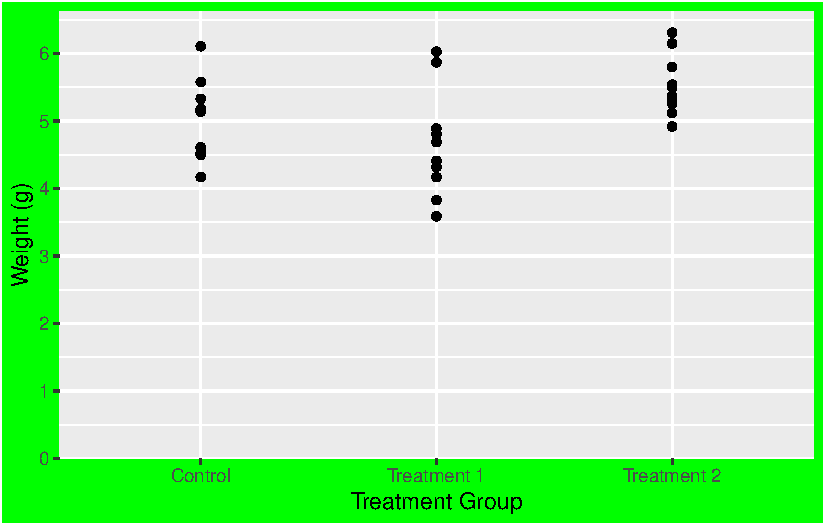
\includegraphics{ggplot2intro_files/figure-pdf/unnamed-chunk-17-1.pdf}

}

\end{figure}

\begin{Shaded}
\begin{Highlighting}[]
\NormalTok{myplot }\SpecialCharTok{+}
  \FunctionTok{theme}\NormalTok{(}\AttributeTok{axis.line =} \FunctionTok{element\_line}\NormalTok{(}\AttributeTok{color =} \StringTok{"red"}\NormalTok{, }\AttributeTok{linewidth =} \DecValTok{3}\NormalTok{))}
\end{Highlighting}
\end{Shaded}

\begin{figure}[H]

{\centering 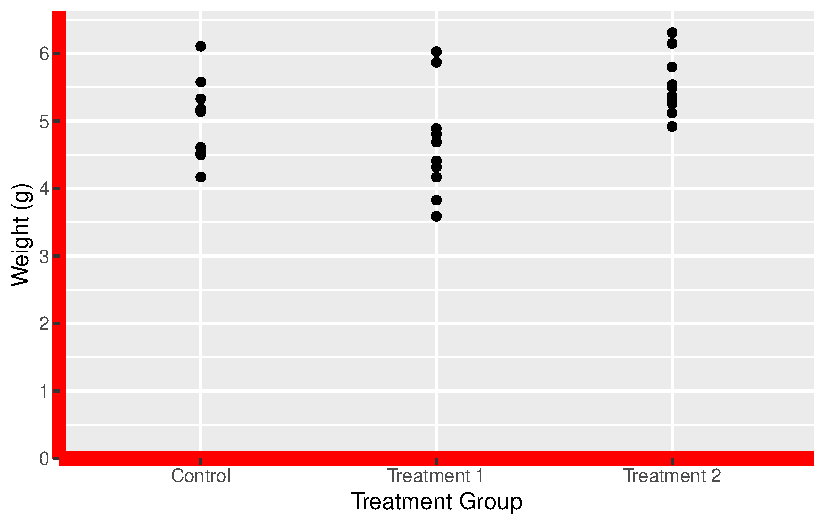
\includegraphics{ggplot2intro_files/figure-pdf/unnamed-chunk-18-1.pdf}

}

\end{figure}

In the first example, we use
\texttt{theme(plot.background\ =\ element\_rect(fill\ =\ "green"))} to
change the plot background to green. In the second example, we use
\texttt{theme(axis.line\ =\ element\_line(color\ =\ "red",\ linewidth\ =\ 3))}
to change the color of the axis lines to red and increase their width.
While these functions may seem a bit cryptic, the good news is that
there are only four different
\href{https://ggplot2.tidyverse.org/reference/element.html}{theme
elements}: \texttt{element\_blank()} draws nothing, and assigns no
space, \texttt{element\_rect()} for borders and backgrounds,
\texttt{element\_line()} for lines and \texttt{element\_text()} for
text.

While the \texttt{theme()} function provides a high level of
customization, it can be time-consuming to manually specify every detail
of your plot. To save time, ggplot2 provides several predefined
``complete themes'' that you can use. These themes have been
professionally designed and provide a quick way to change the overall
appearance of your plot.

The default theme in ggplot2 is \texttt{theme\_grey()}. However, there
are several other themes available, such as \texttt{theme\_bw()},
\texttt{theme\_classic()}, \texttt{theme\_dark()}, and more. Let's take
a look at two of these themes that I personally like:

\begin{Shaded}
\begin{Highlighting}[]
\NormalTok{myplot }\SpecialCharTok{+}
  \FunctionTok{theme\_classic}\NormalTok{()}
\end{Highlighting}
\end{Shaded}

\begin{figure}[H]

{\centering 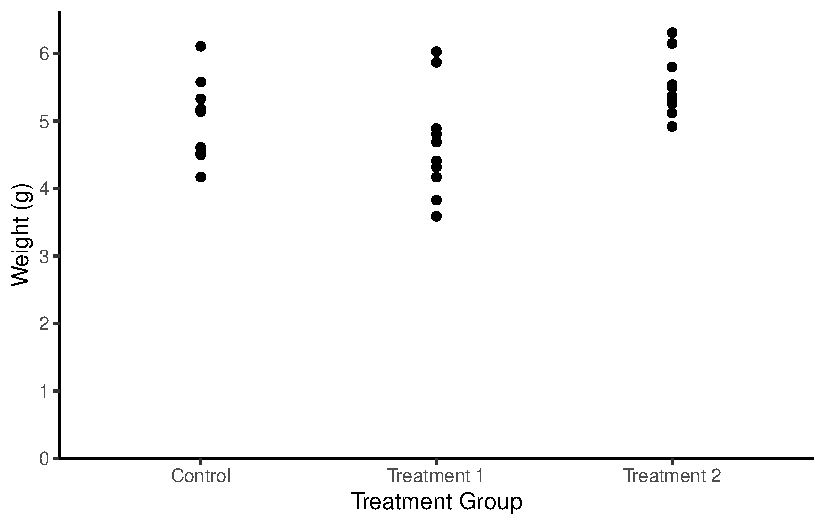
\includegraphics{ggplot2intro_files/figure-pdf/unnamed-chunk-19-1.pdf}

}

\end{figure}

\begin{Shaded}
\begin{Highlighting}[]
\NormalTok{myplot }\SpecialCharTok{+}
  \FunctionTok{theme\_bw}\NormalTok{()}
\end{Highlighting}
\end{Shaded}

\begin{figure}[H]

{\centering 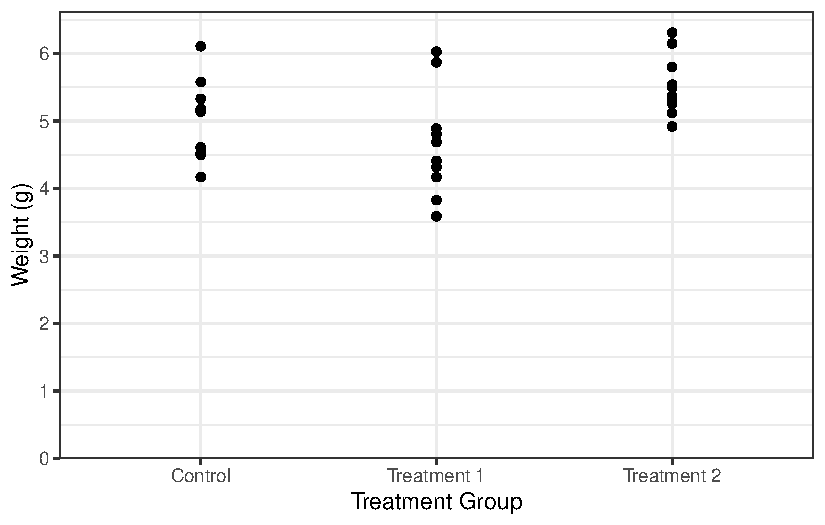
\includegraphics{ggplot2intro_files/figure-pdf/unnamed-chunk-20-1.pdf}

}

\end{figure}

Note that you can also first add a complete \texttt{theme\_*()} and
subsequently change individual aspects of it with via \texttt{theme()}.

Remember, while themes can greatly enhance the aesthetic appeal of your
plots, the most important aspect of any plot is its ability to
accurately and effectively convey information about your data. Always
prioritize clarity and accuracy over aesthetic appeal when creating your
plots.

\begin{tcolorbox}[enhanced jigsaw, left=2mm, title=\textcolor{quarto-callout-tip-color}{\faLightbulb}\hspace{0.5em}{Additional Resources}, toprule=.15mm, colback=white, coltitle=black, opacityback=0, breakable, titlerule=0mm, bottomtitle=1mm, toptitle=1mm, colbacktitle=quarto-callout-tip-color!10!white, arc=.35mm, rightrule=.15mm, bottomrule=.15mm, leftrule=.75mm, colframe=quarto-callout-tip-color-frame, opacitybacktitle=0.6]

\begin{itemize}
\tightlist
\item
  \href{https://ggplot2.tidyverse.org/reference/ggtheme.html}{List of
  all complete themes}
\item
  \href{https://ggplot2.tidyverse.org/reference/theme.html}{Documenation
  of the \texttt{theme()} function}
\end{itemize}

\end{tcolorbox}

We update our \texttt{myplot} according to what we just learned. To get
a better overview, we recreate it from scratch:

\begin{Shaded}
\begin{Highlighting}[]
\NormalTok{myplot }\OtherTok{\textless{}{-}} \FunctionTok{ggplot}\NormalTok{(}\AttributeTok{data =}\NormalTok{ PlantGrowth) }\SpecialCharTok{+}
  \FunctionTok{aes}\NormalTok{(}\AttributeTok{y =}\NormalTok{ weight, }\AttributeTok{x =}\NormalTok{ group) }\SpecialCharTok{+}
  \FunctionTok{geom\_point}\NormalTok{() }\SpecialCharTok{+}
  \FunctionTok{scale\_y\_continuous}\NormalTok{(}
    \AttributeTok{name =} \StringTok{"Weight (g)"}\NormalTok{,}
    \AttributeTok{limits =} \FunctionTok{c}\NormalTok{(}\DecValTok{0}\NormalTok{, }\ConstantTok{NA}\NormalTok{),}
    \AttributeTok{breaks =} \FunctionTok{seq}\NormalTok{(}\DecValTok{0}\NormalTok{, }\DecValTok{6}\NormalTok{),}
    \AttributeTok{expand =} \FunctionTok{expansion}\NormalTok{(}\AttributeTok{mult =} \FunctionTok{c}\NormalTok{(}\DecValTok{0}\NormalTok{, }\FloatTok{0.05}\NormalTok{))}
\NormalTok{  ) }\SpecialCharTok{+}
  \FunctionTok{scale\_x\_discrete}\NormalTok{(}
    \AttributeTok{name =} \StringTok{"Treatment Group"}\NormalTok{,}
    \AttributeTok{labels =} \FunctionTok{c}\NormalTok{(}
      \AttributeTok{ctrl =} \StringTok{"Control"}\NormalTok{, }
      \AttributeTok{trt1 =} \StringTok{"Treatment 1"}\NormalTok{, }
      \AttributeTok{trt2 =} \StringTok{"Treatment 2"}
\NormalTok{    )}
\NormalTok{  ) }\SpecialCharTok{+}
  \FunctionTok{theme\_classic}\NormalTok{()}
\end{Highlighting}
\end{Shaded}

\hypertarget{export}{%
\section{Export}\label{export}}

Once you have created a plot in ggplot2, you may want to export it as an
image file. This can be useful for including the plot in a report, a
presentation, or a website.

In RStudio, you can manually export your plots by clicking on the
`Export' button in the `Plots' pane. This will open a dialog box where
you can choose the format and settings for your exported image.

However, a more flexible and reproducible way to export your plots is by
using the \texttt{ggsave()} function provided by ggplot2. This function
allows you to specify the details of the exported image directly in your
code, ensuring that you can reproduce the exact same image in the
future. The \texttt{ggsave()} function has several arguments that allow
you to specify the details of the exported image:

\begin{Shaded}
\begin{Highlighting}[]
\FunctionTok{ggsave}\NormalTok{(}
  \AttributeTok{filename =} \StringTok{"myplot.png"}\NormalTok{, }
  \AttributeTok{plot =}\NormalTok{ myplot, }
  \AttributeTok{path =} \StringTok{"C:/Users/YourName/Documents"}\NormalTok{, }
  \AttributeTok{scale =} \DecValTok{1}\NormalTok{, }
  \AttributeTok{width =} \DecValTok{6}\NormalTok{, }
  \AttributeTok{height =} \DecValTok{4}\NormalTok{, }
  \AttributeTok{units =} \StringTok{"cm"}\NormalTok{, }
  \AttributeTok{dpi =} \DecValTok{300}
\NormalTok{)}
\end{Highlighting}
\end{Shaded}

\begin{itemize}
\item
  \textbf{filename:} This is the name of the file that you want to
  create. You should include the file extension (e.g., .png, .jpg, .pdf)
  in the filename. The file extension determines the format of the
  exported image.
\item
  \textbf{plot:} This is the plot that you want to save. If you don't
  specify a plot, ggsave() will save the last plot that you created.
\item
  \textbf{path:} This is the directory where you want to save the file.
  If you don't specify a path, ggsave() will save the file in your
  current working directory.
\item
  \textbf{scale:} This is a scaling factor that is applied to the text
  and elements of the plot. A scale of 1 means that the plot is saved at
  its original size. A scale of 2 means that the plot is saved at twice
  its original size.
\item
  \textbf{width, height:} These are the dimensions of the exported
  image. You can specify the dimensions in any units that you like
  (e.g., inches, cm, mm).
\item
  \textbf{units:} This is the units in which the width and height are
  specified. The default is ``in'' for inches, but you can also use
  ``cm'' for centimeters, ``mm'' for millimeters, or ``px'' for pixels.
\item
  \textbf{dpi:} This is the resolution of the exported image in dots per
  inch. A higher dpi will result in a higher-quality image, but the file
  size will also be larger. The default dpi is 300, which is suitable
  for most purposes.
\end{itemize}

In this example, we are saving \texttt{myplot} as a PNG file named
``myplot.png'' in the Documents directory. The plot is saved at its
original size (scale = 1) and the dimensions of the image are 6 cm by 4
cm. The resolution of the image is 300 dpi.

\begin{tcolorbox}[enhanced jigsaw, left=2mm, title=\textcolor{quarto-callout-tip-color}{\faLightbulb}\hspace{0.5em}{Tip}, toprule=.15mm, colback=white, coltitle=black, opacityback=0, breakable, titlerule=0mm, bottomtitle=1mm, toptitle=1mm, colbacktitle=quarto-callout-tip-color!10!white, arc=.35mm, rightrule=.15mm, bottomrule=.15mm, leftrule=.75mm, colframe=quarto-callout-tip-color-frame, opacitybacktitle=0.6]

If you want to open the image file you've just created directly on your
computer, you can use the \texttt{system()} function in R. For instance,
\texttt{system(\textquotesingle{}open\ "FILENAME"\textquotesingle{})}
will open the specified file. So, in our case, running
\texttt{system(\textquotesingle{}open\ "C:/Users/YourName/Documents/myplot.png"\textquotesingle{})}
will open the PNG file we've just created, and it will do so outside of
RStudio.

I find this approach preferable to viewing my ggplot in RStudio's
Plots-pane, because it gives you a more accurate preview of how your
plot will look in its final context. The preview in RStudio actually
doesn't do this, because the scale and size of the plot adjusts to the
size you dragged the Plots-pane to.

Here is a
\href{https://gist.github.com/SchmidtPaul/5cd96b53449f5f50cbda725d4cdacf9b}{gist}
of how I used to apply this approach, but nowadays I wrapped all of this
into
\href{https://schmidtpaul.github.io/BioMathR/reference/gg_export.html}{my
own function}.

\end{tcolorbox}

\hypertarget{color-shape-and-more}{%
\section{Color, Shape and More}\label{color-shape-and-more}}

In ggplot2, the aesthetics of your plot, such as color and shape, can be
adjusted to enhance the visual representation of your data. In this
section, we will explore how to manipulate these aesthetics using the
\texttt{geom\_point()} function.

First, let's recreate our \texttt{myplot} object, but this time without
the \texttt{geom\_point()} layer. This will provide us with a clean
slate to experiment with:

\begin{Shaded}
\begin{Highlighting}[]
\NormalTok{myplot }\OtherTok{\textless{}{-}} \FunctionTok{ggplot}\NormalTok{(}\AttributeTok{data =}\NormalTok{ PlantGrowth) }\SpecialCharTok{+}
  \FunctionTok{aes}\NormalTok{(}\AttributeTok{y =}\NormalTok{ weight, }\AttributeTok{x =}\NormalTok{ group) }\SpecialCharTok{+}
  \FunctionTok{scale\_y\_continuous}\NormalTok{(}
    \AttributeTok{name =} \StringTok{"Weight (g)"}\NormalTok{,}
    \AttributeTok{limits =} \FunctionTok{c}\NormalTok{(}\DecValTok{0}\NormalTok{, }\ConstantTok{NA}\NormalTok{),}
    \AttributeTok{breaks =} \FunctionTok{seq}\NormalTok{(}\DecValTok{0}\NormalTok{, }\DecValTok{6}\NormalTok{),}
    \AttributeTok{expand =} \FunctionTok{expansion}\NormalTok{(}\AttributeTok{mult =} \FunctionTok{c}\NormalTok{(}\DecValTok{0}\NormalTok{, }\FloatTok{0.05}\NormalTok{))}
\NormalTok{  ) }\SpecialCharTok{+}
  \FunctionTok{scale\_x\_discrete}\NormalTok{(}
    \AttributeTok{name =} \StringTok{"Treatment Group"}\NormalTok{,}
    \AttributeTok{labels =} \FunctionTok{c}\NormalTok{(}
      \AttributeTok{ctrl =} \StringTok{"Control"}\NormalTok{, }
      \AttributeTok{trt1 =} \StringTok{"Treatment 1"}\NormalTok{, }
      \AttributeTok{trt2 =} \StringTok{"Treatment 2"}
\NormalTok{    )}
\NormalTok{  ) }\SpecialCharTok{+}
  \FunctionTok{theme\_classic}\NormalTok{()}
\end{Highlighting}
\end{Shaded}

\hypertarget{general-aesthetic-modifications}{%
\subsection{General Aesthetic
Modifications}\label{general-aesthetic-modifications}}

To show you what is possible with \texttt{geom\_point()}, let's create
two new plots. In the first plot, we will set the color of the points to
orange. In the second plot, we will modify several aspects of the
points, including color, shape, size, and transparency.

\begin{Shaded}
\begin{Highlighting}[]
\NormalTok{myplot }\SpecialCharTok{+}
  \FunctionTok{geom\_point}\NormalTok{(}\AttributeTok{color =} \StringTok{"orange"}\NormalTok{)}
\end{Highlighting}
\end{Shaded}

\begin{figure}[H]

{\centering 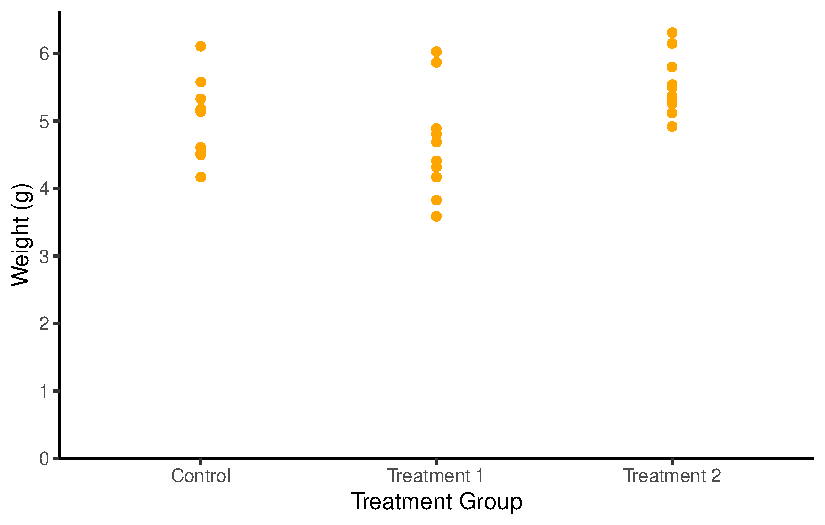
\includegraphics{ggplot2intro_files/figure-pdf/unnamed-chunk-24-1.pdf}

}

\end{figure}

\begin{Shaded}
\begin{Highlighting}[]
\NormalTok{myplot }\SpecialCharTok{+}
  \FunctionTok{geom\_point}\NormalTok{(}
    \AttributeTok{color =} \StringTok{"purple"}\NormalTok{, }
    \AttributeTok{shape =} \DecValTok{18}\NormalTok{, }
    \AttributeTok{size =} \DecValTok{3}\NormalTok{, }
    \AttributeTok{alpha =} \FloatTok{0.5}
\NormalTok{  )}
\end{Highlighting}
\end{Shaded}

\begin{figure}[H]

{\centering 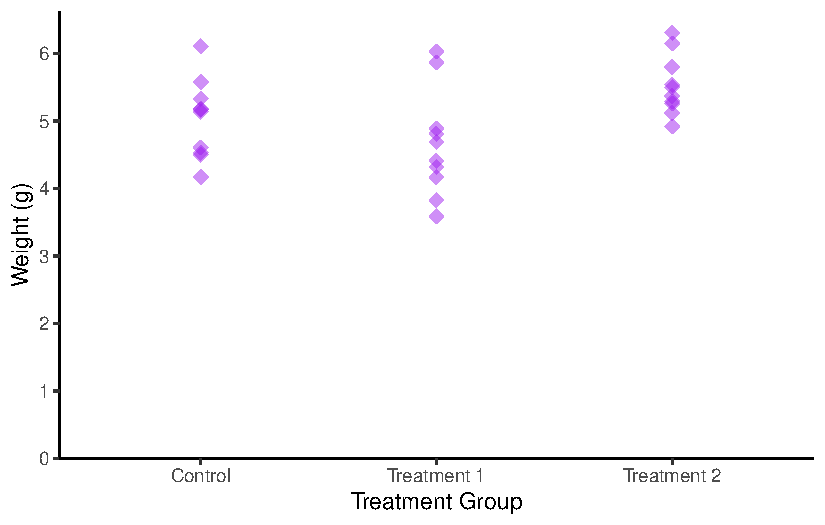
\includegraphics{ggplot2intro_files/figure-pdf/unnamed-chunk-25-1.pdf}

}

\end{figure}

In the first plot, we use color = ``orange'' inside the geom\_point()
function. This sets the color of all points to orange.

In the second plot, we modify several aspects of the points:

\begin{itemize}
\tightlist
\item
  color = ``purple'' sets the color of the points to purple. shape = 18
  changes the shape of the points. ggplot2 includes several different
  shapes that you can use. The number 18 corresponds to a filled diamond
  shape.
\item
  size = 3 increases the size of the points. The size is measured in mm.
\item
  alpha = 0.5 sets the transparency of the points. The alpha value
  ranges from 0 (completely transparent) to 1 (completely opaque).
\end{itemize}

These modifications allow us to customize the appearance of the points
to suit our preferences and the needs of our data.

\hypertarget{aesthetic-mapping-with-aes}{%
\subsection{Aesthetic Mapping with
aes()}\label{aesthetic-mapping-with-aes}}

\hypertarget{end}{%
\section*{End}\label{end}}
\addcontentsline{toc}{section}{End}

\hypertarget{refs}{}
\begin{CSLReferences}{1}{0}
\leavevmode\vadjust pre{\hypertarget{ref-heiss_2023}{}}%
Heiss, Andrew. 2023. {``{D}ata {V}isualization with {R} - {D}ata
{V}isualization.''} \url{https://datavizs23.classes.andrewheiss.com/}.

\leavevmode\vadjust pre{\hypertarget{ref-scherer_2022}{}}%
Scherer, Cédric. 2022a. {``A Ggplot2 Tutorial for Beautiful Plotting in
r.''} \emph{Cédric Scherer Blog}.
\url{https://www.cedricscherer.com/2019/08/05/a-ggplot2-tutorial-for-beautiful-plotting-in-r/}.

\leavevmode\vadjust pre{\hypertarget{ref-scherer_2022b}{}}%
---------. 2022b. {``{G}raphic {D}esign with Ggplot2 - {G}raphic
{D}esign with Ggplot2.''} \emph{Rstudio::conf(2022) Workshop}.
\url{https://rstudio-conf-2022.github.io/ggplot2-graphic-design/}.

\leavevmode\vadjust pre{\hypertarget{ref-wickham_2017}{}}%
Wickham, Hadley, and Garrett Grolemund. 2017. \emph{R for Data Science:
Import, Tidy, Transform, Visualize, and Model Data}. 1st ed. O'Reilly
Media, Inc. \url{https://r4ds.had.co.nz/}.

\leavevmode\vadjust pre{\hypertarget{ref-wilke_2019}{}}%
Wilke, Claus O. 2019. \emph{{Fundamentals of data visualization}}.
{O'Reilly Media}. \url{https://clauswilke.com/dataviz/}.

\end{CSLReferences}



\end{document}
